\begin{center}
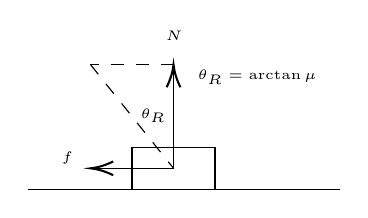
\begin{tikzpicture}[x=0.75pt,y=0.75pt,yscale=-1,xscale=1]
%uncomment if require: \path (0,300); %set diagram left start at 0, and has height of 300

%Straight Lines [id:da524357483065941] 
\draw    (140,130) -- (290,130) ;
%Shape: Rectangle [id:dp1562964743350983] 
\draw   (190,110) -- (230,110) -- (230,130) -- (190,130) -- cycle ;
%Straight Lines [id:da659959210580102] 
\draw    (210,120) -- (210,72) ;
\draw [shift={(210,70)}, rotate = 90] [color={rgb, 255:red, 0; green, 0; blue, 0 }  ][line width=0.75]    (10.93,-3.29) .. controls (6.95,-1.4) and (3.31,-0.3) .. (0,0) .. controls (3.31,0.3) and (6.95,1.4) .. (10.93,3.29)   ;
%Straight Lines [id:da5537782404532552] 
\draw    (210,120) -- (172,120) ;
\draw [shift={(170,120)}, rotate = 360] [color={rgb, 255:red, 0; green, 0; blue, 0 }  ][line width=0.75]    (10.93,-3.29) .. controls (6.95,-1.4) and (3.31,-0.3) .. (0,0) .. controls (3.31,0.3) and (6.95,1.4) .. (10.93,3.29)   ;
%Straight Lines [id:da5271088999254347] 
\draw  [dash pattern={on 4.5pt off 4.5pt}]  (210,70) -- (170,70) ;
%Straight Lines [id:da223898729028551] 
\draw  [dash pattern={on 4.5pt off 4.5pt}]  (170,70) -- (210,120) ;

% Text Node
\draw (155,111) node [anchor=north west][inner sep=0.75pt]  [font=\tiny] [align=left] {$\displaystyle f$};
% Text Node
\draw (205,52.5) node [anchor=north west][inner sep=0.75pt]  [font=\tiny] [align=left] {$\displaystyle N$};
% Text Node
\draw (193,90) node [anchor=north west][inner sep=0.75pt]  [font=\tiny] [align=left] {$\displaystyle \theta_R $};
% Text Node
\draw (220.5,71.5) node [anchor=north west][inner sep=0.75pt]  [font=\tiny] [align=left] {$\displaystyle \theta_R =\arctan \mu $};


\end{tikzpicture}

\end{center}